\subsection{Display > Render to File}
\label{subsection:renderToFile}

\index{capture d'�cran}
Effectue une capture d'�cran du contexte actif dans un fichier BMP.
Cette fonction offre la possibilit� d'appliquer un facteur de zoom au moment
de la capture, via la fen�tre pr�sent�e en figure \ref{fig:snapshotZoom}.

\begin{figure}[!htb]
\begin{center}
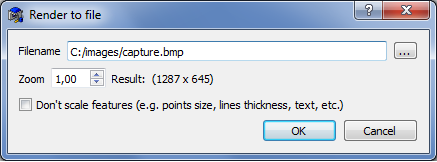
\includegraphics[width=0.3\textwidth]{images/Partie3_Fonctions/snapshotZoom}
\caption{\label{fig:snapshotZoom}Fen�tre de zoom pour la capture du contexte graphique courant}
\end{center}
\end{figure}